\documentclass{beamer} 
\usetheme{default} 
\usecolortheme{albatross}
\setbeamercovered{transparent}
%\useoutertheme{umbcfootline}  


\usepackage[spanish]{babel}
%\usepackage[latin1]{inputenc}
\usepackage[utf8x]{inputenc}
\usepackage{hyperref}
\usepackage{color}



%\usepackage{multicol}
\usepackage{multicol}


\title{POLIMORFISMO E INTERFACES}

\author{Manuel J. Molino Milla \and Luis Molina Garzón}

\date{\today} %

\institute{IES Virgen del Carmen \and Departamento de Informática}




%\beamerdefaultoverlayspecification{<+->}

\begin{document}


\begin{frame}
  \titlepage
\end{frame}

\begin{frame}
    \frametitle{Logo}
\begin{figure}

\includegraphics[scale=1]{imagenes/logo.jpeg} 
\caption{Logo Java}
\end{figure}
\end{frame}

\begin{frame}
  \frametitle{Contenido}
  \tableofcontents[pausesections]
\end{frame}

\section{POLIMORFISMO}
\begin{frame}
\frametitle{Introducción}
\begin{scriptsize}
\begin{block}{Caracteristicas de POO}
\begin{itemize}[<+->]
\item ENCAPSULACIÓN.
\item HERENCIA.
\item POLIMORFISMO
\end{itemize}
\end{block}
\pause
\begin{block}{Herencia}
\begin{itemize}[<+->]
\item Una clase define un nuevo tipo.
\item Una subclase define un \emph{subtipo}
\item Una superclase define un \emph{supertipo}
\end{itemize}
\end{block}
\pause
\begin{block}{Relaciones de herencia}
\begin{itemize}[<+->]
\item Las relaciones de herencia permiten a una subclase a heredar características de la superclase.
\item Además añade nuevas características.
\item Una subclase es una especialización de una superclase.
\item Cada instancia de la subclase a su vez es una instancia de la superclase.
\item Pero \emph{NO} al revés.
\end{itemize}
\end{block}
\end{scriptsize}
\end{frame}

\begin{frame}
\frametitle{UML herencia}
\begin{figure}
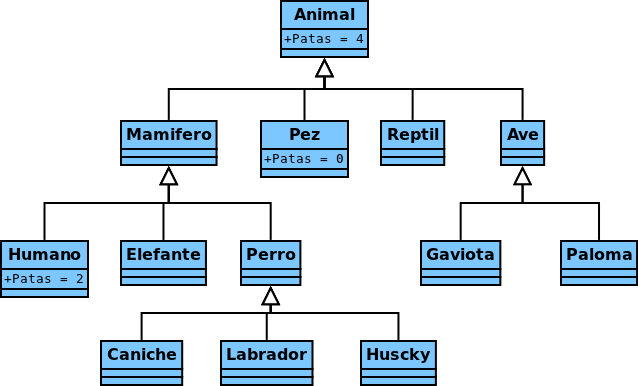
\includegraphics[scale=0.3]{imagenes/herencia1.png}
\end{figure}
\begin{itemize}[<+->]
\item Un mamífero es un animal, pero un animal no es un mamífero.
\item Un humano es un mamífero, pero un mamifero no es un humano.
\item Un humano es un animal, pero un animal no es un humano.
\end{itemize}
\end{frame}


\begin{frame}[fragile]
\frametitle{Polimorfismo}
\begin{itemize}[<+->]
\item El polimorfismo nos permite programar en forma general
\item Nos permite escribir programas que procesen objetos que compartan la misma superclase en una jerarquía de clases
\item Como si todos fueran objetos de la superclase
\item Con el polimorfismo podemos diseñar e implementar sistemas que puedan extenderse con facilidad.
\item Pueden agregarse nuevas clases con sólo modificar un poco (o nada) las porciones generales de la aplicación.
\item Siempre y cuando las nuevas clases sean parte de la jerarquía de herencia que la aplicación procesa en forma genérica.
\end{itemize}
\end{frame}


\begin{frame}
\frametitle{}
\begin{figure}
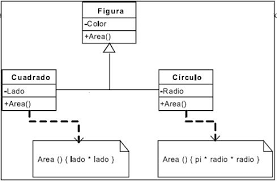
\includegraphics[scale=0.8]{imagenes/figuras.png}
\end{figure}
\end{frame}


\begin{frame}[fragile]
\frametitle{Ejemplo de polimorfismo}
\begin{scriptsize}
\begin{verbatim}
public class PolimorfismoDemo {
  public static void main(String[] args) {
     displayFigura(new Circulo("rojo"));
     displayFigura(new Cuadrardo("amarillo"));
  }
/** Display geometric object properties */

   public static void displayFigura(Figura object) {
   //el método area() se define en la clase padre
   //y se sobrescribe en las clases hijas
    System.out.println("Area del objeto: "+object.area());
   }
}
\end{verbatim}
\pause
\begin{itemize}[<+->]
\item El método \emph{displayFigura} tiene como parámetro \emph{Figura object}
\item El parámetro que se le pasa es un objeto de la superclase.
\item Pero como cualquier objeto de la subclase es tambien un objeto de la superclase.
\item Podemos pasar sin ningún problema objetos de tipo \emph{Circulo} o tipo \emph{Cuadrado}
\item Pues en la definición se habrán creado las clases como subclases de \emph{Figura}
\item Ahora sería fácil añadir una clase \emph{Triangulo}
\end{itemize}
\end{scriptsize}
\end{frame}

\section{LIGADURA DINAMICA}
\begin{frame}
\frametitle{Ligadura dinámica}
\begin{itemize}[<+->]
\item Un método puede ser definido en una superclase y sobrescrito en una subclase.
\item Ejemplo el método \emph{subString()}
\end{itemize}
\pause
\begin{quote}
Object o = new GeometricObject();\\
System.out.println(o.toString());
\end{quote}
\pause
\begin{itemize}[<+->]
\item ¿Cual metodo se invoca? Ya que \emph{o} es tipo \emph{Object}
\item Hay que distinguir entre \emph{tipo declarado} y \emph{tipo actual}
\item \emph{o} es declarado como \emph{Object} pero es de tipo \emph{GeometricObject}
\item A esto se le denomina ligadura dinámica.
\item En compilación se le guarda una posición de memoria para un objeto de tipo \emph{Object}
\item En tiempo de ejecución se reservar espacio en el montículo para un objeto de tipo \emph{GeometricObject}
\end{itemize}
\end{frame}

\begin{frame}
\frametitle{Ligadura dinámica}
\begin{figure}
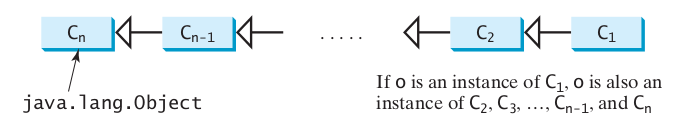
\includegraphics[scale=0.5]{imagenes/polimorfismo1.png}
\end{figure}
\pause
\begin{itemize}[<+->]
\item En este caso $C_{n}$ es un objeto de la clase \emph{Object}
\item La JVM busca el método invocado desde las clases $C_{1}$,$C_{2}$, \dots, $C_{n}$ hasta localizarlo.
\end{itemize}
\end{frame}

\begin{frame}[fragile]
\frametitle{Ejemplo ligadura dinámica}
\begin{multicols}{2}
\begin{tiny}
\begin{verbatim}
public class DynamicBindingDemo {
  public static void main(String[] args) {
    m(new GraduateStudent());
    m(new Student());
    m(new Person());
    m(new Object());
   }
  public static void m(Object x) {
    System.out.println(x.toString());
    }
}
class GraduateStudent extends Student {}

class Student extends Person {
  public String toString() {
    return "Student";
  }
}
class Person extends Object {
  public String toString() {
    return "Person";
  }
}
\end{verbatim}

\pause
\emph{La salida es:}\\
Student\\
Student\\
Person\\
java.lang.Object$@$135fbaa4\\
\end{tiny}
\emph{OJO, hay un método sobrescrito \emph{toString()}}
\end{multicols}
\end{frame}


\section{CASTING}
\begin{frame}
\frametitle{Casting}
\begin{itemize}[<+->]
\item En el ejemplo anterior podíamos haber hecho:
\item \emph{Object o = new Student();}
\item Porque un objeto de tipo \emph{Student} es un objeto de tipo \emph{Object}
\item Ahora esto causa un error: \emph{Student b = o;}
\item Porque un objeto de tipo \emph{Object} no siempre es de tipo \emph{Student}
\item La única manera de susanar el error es hacer un \emph{casting}
\item \emph{Student b = (Student)o; // Explicit casting}
\item El \emph{upcasting} es automática y el \emph{downcasting} hay que especificarlo.
\item Si un objeto de la superclase no es una instancia de la subclase ocuerre una \emph{ClassCastException}
\item En este caso no ocurre pues hemos definido al principio:
\item \emph{Object o = new Student();}
\end{itemize}
\end{frame}
\section{OPERADOR INSTANCEOF}
\begin{frame}[fragile]
\frametitle{Operador instanceof}
\begin{verbatim}
Object miObjeto = new Circulo();
..............................
if (miObjeto instanceof Circulo) {
System.out.println("El diametro del círculo es " +
((Circle)miObjeto) .getDiametro());
...
}
\end{verbatim}
\begin{footnotesize}
\begin{itemize}[<+->]
\item ¿Por qué es necesario el casting? \emph{((Circle)miObjeto) .getDiametro());}
\item Porque miObjeto es declarado como \emph{Object}.
\item Y el tipo declarado decide el tipo de método a emplear en tiempo de compilación.
\item Usando \emph{miObjeto.getDiametro()} causa un error de compilación, porque la clase \emph{Object} no tiene el método \emph{getDiametro()}.
\item ¿Por qué no se define la variable \emph{miObjeto} como tipo \emph{Circulo}?
\item \textbf{Porque en POO es una buena práctica definir la variable del tipo de la \emph{superclase} la cuál puede aceptar un valor de cualquier subtipo.}
\end{itemize}
\end{footnotesize}
\end{frame}

\begin{frame}
\frametitle{Ejemplo}
\begin{quote}
List$<$String$>$ lista = new ArrayList$<$String$>$();
\end{quote}
\pause
\begin{quote}
Set$<$String$>$ conjunto = new HashSet$<$String$>$();
\end{quote}
\end{frame}


\begin{frame}[fragile]
\frametitle{Ejemplo de instanceof}
\begin{verbatim}
public class Empleado { .... }
public class Jefe extends Empleado { .... }
public class ObreroEspecializado extendes Empleado { .... }
.....
   public void metodo (Empleado e){
   if (e instanceof Jefe){
      //Obtiene beneficios por objetivos
   }
   else if (e instanceof ObreroEspecializado){
      //Obtiene beneficios por horas extras
   }
   else {
   		//No obtiene beneficios
\end{verbatim}
\emph{El hecho de haber definido \emph{metodo(Empleado e)} nos permite implementar un único método para todas las subclases de \emph{Empleado} y no tener que crear un método para cada subclase}
\end{frame}

\section{CLASES ABSTRACTAS}
\begin{frame}[fragile]
\frametitle{Introducción a las clases abstractas}
\begin{small}
\begin{itemize}[<+->]
\item Hay ocasiones, cuando se desarrolla una jerarquía de clases en que algún comportamiento está presente en todas ellas pero se materializa de forma distinta para cada una.
\item Por ejemplo, pensemos en una estructura de clases para manipular figuras geométricas.
\item Podríamos pensar en tener una clase genérica, que podría llamarse FiguraGeometrica y una serie de clases que extienden a la anterior que podrían ser Circulo, Poligono,\dots
\item Podría haber un método dibujar dado que sobre todas las figuras puede llevarse a cabo esta acción.
\item Pero las operaciones concretas para llevarla a cabo dependen del tipo de figura en concreto (de su clase).
\item Por otra parte la acción dibujar no tiene sentido para la clase genérica FiguraGeometrica, porque esta clase representa una abstracción del conjunto de figuras posibles.
\item Para resolver esta problemática Java proporciona las clases y métodos abstractos
\end{itemize}
\end{small}
\end{frame}

\begin{frame}[fragile]
\frametitle{Ejemplo}
\begin{scriptsize}
\begin{verbatim}
abstract class FiguraGeometrica {
    . . .
    abstract void dibujar();
    . . .
}

class Circulo extends FiguraGeometrica {
    . . .
    void dibujar() {
        // codigo para dibujar Circulo
        . . .
    }
} 
\end{verbatim}
\pause
\begin{itemize}[<+->]
\item  Un método abstracto es un método declarado en una clase para el cual esa clase no proporciona la implementación (el código).
\item Una clase abstracta es una clase que tiene al menos un método abstracto.
\item Una clase que extiende de una clase abstracta debe implementar los métodos abstractos (escribir el código)
\item O bien volverlos a declarar como abstractos, con lo que ella misma se convierte también en clase abstracta. 
\end{itemize}
\end{scriptsize}
\end{frame}

 
\begin{frame}[fragile]
\frametitle{Referencias y objetos abstractos}
\begin{itemize}[<+->]
\item Se pueden crear referencias a clases abstractas como cualquier otra.
\item No hay ningún problema en poner: \emph{FiguraGeometrica figura;}
\item Sin embargo una clase abstracta no se puede instanciar, es decir, no se pueden crear objetos de una clase abstracta. 
\item El compilador producirá un error si se intenta:
\item \emph{FiguraGeometrica figura = new FiguraGeometrica();}
\item Sin embargo utilizando el \textbf{up-casting}: 
\item \emph{FiguraGeometrica figura = new Circulo(\dots); figura.dibujar();}
\end{itemize}
\end{frame}

\begin{frame}[fragile]
\frametitle{Ejemplo}
\begin{figure}
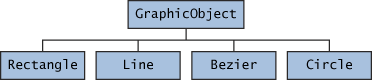
\includegraphics[scale=0.5]{imagenes/abstract1.png}
\end{figure}
\begin{tiny}
\begin{multicols}{2}
\begin{verbatim}
abstract class GraphicObject {
    int x, y;
    ...
    void moveTo(int newX, int newY) {
        ...
    }
    abstract void draw();
    abstract void resize();
}







class Circle extends GraphicObject {
    void draw() {
        ...
    }
    void resize() {
        ...
    }
}
class Rectangle extends GraphicObject {
    void draw() {
        ...
    }
    void resize() {
        ...
    }
}
\end{verbatim}
\end{multicols}
\end{tiny}
\end{frame}



\begin{frame}[fragile]
\frametitle{Caracteristicas de las clases abstractas}
\begin{footnotesize}
\begin{itemize}[<+->]
\item Que una clase abstracta no pueda ser instanciada no implica que no pueda tener un constructor.
\item Si no definimos un constructor, existe el constructor por defecto.
\item El sentido del constructor en las clases abstractas obliga a \emph{settear} los valores de los atributos de la clase base (clase abstracta).
\end{itemize}
\end{footnotesize}
\pause
\begin{tiny}
\begin{verbatim}
        public abstract class FiguraGeometrica
         {
           private String nombre;
           public abstract double area ();

         public FiguraGeometrica (String nombre)
           {
             this.nombre = nombre;
           }
         public String toString ()
           {
             return this.nombre + " area: " + this.area ();
           }
         public String getNombre ()
           {
             return this.nombre;
           }
         public void setNombre (String nombre)
           {
             this.nombre = nombre;
           }
         public abstract double getArea(){}
         }    
\end{verbatim}
\end{tiny}
\end{frame}

\begin{frame}[fragile]
\frametitle{Siguiendo el ejemplo}
\begin{multicols}{2}
\begin{tiny}
\begin{verbatim}







import java.lang.Math;
public class Circulo extends FiguraGeometrica
{
  private int radio;
  public Circulo (int r)
  {
    super ("Círculo");
    this.radio = r;
  }
  public double area ()
  {
    return Math.PI * radio * radio;
  }
}







public class Cuadrado extends FiguraGeometrica
{
  private int arista;
  public Cuadrado (int a)
  {
    super ("Cuadrado");
    this.arista = a;
  }
  public double area ()
  {
    return arista * arista;
  }
}


public class TestFiguraGeometricas
{
  public static void main (String[]arg)
  {
    Circulo c = new Circulo (2);
    System.out.println ("Figura: " + c.getNombre ());
    System.out.println ("Área: " + c.area ());
    Cuadrado cu = new Cuadrado (2);
    System.out.println ("Figura: " + cu.getNombre ());
    System.out.println ("Área: " + cu.area ());
  }
}

\end{verbatim}
\end{tiny}
\end{multicols}
\end{frame}

\section{INTERFACES}

\begin{frame}
\frametitle{Interfaces}
\begin{itemize}[<+->]
\item Una interfaz es similar a las clases abstractas.
\item Establece la apariencia que tendrán todas las clases que \textbf{implementen} esa interfaz.
\item Permite al creador establecer la forma de una clase: \emph{nombres de metodos, listas de parametros, y tipos de retorno, pero no cuerpos de metodo.}
\item Una interfaz tambien puede tener campos, peros estos son implicitamente \textbf{estaticos y constantes}.
\item Para crear una interfaz usamos la palabra \emph{interface} en vez de \textbf{class}.
\item Para hacer que una clase se ajuste a una interfaz particular se usa la palabra clave \emph{implements}.
\item Mientras que la herencia una clase \textbf{solo} puede tener \textbf{una} clase padre, en este caso una clase puede implementar \textbf{varias} interfaces
\end{itemize}
\end{frame}



\begin{frame}[fragile]
\frametitle{Interfaces}
Una interface se declara:
{\color{yellow}
\begin{verbatim}
interface nombre_interface {
    tipo_retorno nombre_metodo ( lista_argumentos ) ;
    . . . 
}
\end{verbatim}}
\pause
Por ejemplo:
\begin{footnotesize}
{\color{yellow}
\begin{verbatim}
interface InstrumentoMusical {
    void tocar();
    void afinar();
    String tipoInstrumento();
}
\end{verbatim}}
\end{footnotesize}
\pause
Y una clase que implementa la interface:
\begin{scriptsize}
{\color{yellow}
\begin{verbatim}
class InstrumentoViento implements InstrumentoMusical {
      void tocar() { . . . };
      void afinar() { . . .};
      String tipoInstrumento() {}
}
class Guitarra extends InstrumentoViento {
      String tipoInstrumento() {
      return "Guitarra";
      }
}   
\end{verbatim}}
\end{scriptsize}
\end{frame}


\begin{frame}[fragile]
\frametitle{Referencias a Interfaces}
Es posible crear referencias a interfaces, pero las interfaces no pueden ser instanciadas. Una referencia a una interface puede ser asignada a cualquier objeto que implemente la interface. Por ejemplo:
{\color{yellow}
\begin{verbatim}
InstrumentoMusical instrumento = new Guitarra();
instrumento.play();
System.out.prinln(instrumento.tipoInstrumento());

//error.No se puede instanciar:
InstrumentoMusical i2 = new InstrumentoMusical(); 
\end{verbatim}}
\end{frame}

\begin{frame}[fragile]
\frametitle{Extensión de interfaces}
Las interfaces pueden extender otras interfaces y, a diferencia de las clases, una interface puede extender más de una interface. La sintaxis es:
{\color{cyan}
\begin{verbatim}
interface nombre_interface  extends nombre_interface, ...{
    tipo_retorno nombre_metodo ( lista_argumentos ) ;
    . . . 
}
\end{verbatim}}
\end{frame}


\begin{frame}[fragile]
\frametitle{Agrupaciones de constantes}
{\color{yellow}
\begin{verbatim}
public interface Meses {
 int ENERO = 1 , FEBRERO = 2 . . . ;
 String [] NOMBRES_MESES = { " " , "Enero", "Febrero",...};
}
\end{verbatim}}
\pause
Esto puede usarse simplemente:
{\color{purple}
\begin{verbatim}
System.out.println(Meses.NOMBRES_MESES[ENERO]);
\end{verbatim}}
\end{frame}

\begin{frame}[fragile]
\frametitle{Cosas importantes sobre interfaces}
\begin{itemize}[<+->]
\item     Todos los métodos de una interfaz son implícitamente \textbf{public abstract}, no es necesario especificarlo en la declaración del mismo.
\item  Todas las variables y atributos de una interfaz son implícitamente constantes (\textbf{public static final}), no es necesario especificarlo en la declaración del misma
\item  Los métodos de una interfaz no pueden ser: static o final.
\item  Una interfaz puede heredar (\textbf{extends}) de una o más interfaces.
\item  Una interfaz \textbf{no} puede heredar de otro elemento que no sea una interfaz.
\item  Una interfaz no puede implementar (\textbf{implements}) otra interfaz.
\item  Una interfaz debe ser declarada con la palabra clave \textbf{interface}.
\item  Una interfaz puede ser public o package (valor por defecto). 
\end{itemize}

\end{frame}

\begin{frame}[fragile]
\frametitle{Interfaces en Java 8}
\begin{itemize}[<+->]
\item Java 8 incluye el método \emph{default} que se puede implementar en la clase interfaz. 
\item Su implementación será común para todas las clases que implementen esa interface
\item Ese método puede sobreescribirse en las clases que implementen esa interfaz.
\item También pueden aparecer métodos estáticos implementados, pero éstos NO se pueden sobreescribir.
\end{itemize}
\end{frame}

\begin{frame}[fragile]
\frametitle{Interfaces en Java 8}
\framesubtitle{Método \emph{default}}
\begin{verbatim}
public interface Interface1 {

  void method1(String str);
	
  default void log(String str){
    System.out.println("I1 logging::" + str);
  }
}
\end{verbatim}
\pause
El método \emph{log} se puede sobrescribir sin problema.
\end{frame}

\begin{frame}[fragile]
\frametitle{Interfaces en Java 8}
\framesubtitle{Métodos estáticos}
\begin{small}
\begin{verbatim}
public interface MyData {

  default void print(String str) {
    if (!isNull(str))
      System.out.println("MyData Print::" + str);
  }

  static boolean isNull(String str) {
    System.out.println("Interface Null Check");

    return str == null ? true : "".equals(str) ? true : false;
  }
}
\end{verbatim}
\end{small}
\pause
El método \emph{isNull} \textbf{NO} se puede sobrescribir.
\end{frame}

\begin{frame}[fragile]
\frametitle{Interfaces en Java 8}
\framesubtitle{Interfaces funcionales}
\begin{footnotesize}

INTERFAZ:
\begin{verbatim}
public interface InterfazFuncional {
	
  double operacionAritmetica(double x, double y);

}

\end{verbatim}
USO DE LA INTERFAZ:
\begin{verbatim}
public class Principal {
  public static void main(String[] args) {
		
    InterfazFuncional suma = (x,y) -> x + y;
    InterfazFuncional multiplicacion = (x,y) -> x * y;
    double sumaValores = 
      suma.operacionAritmetica(2,3);
    double multiplicarValores = 
      multiplicacion.operacionAritmetica(2, 3);
		
  }
}
\end{verbatim}

\end{footnotesize}
\end{frame}


\begin{frame}
\frametitle{Interfaces comunes en Java}
\begin{tiny}
\begin{block}{Comparable}
Se utiliza para permitir que los objetos de una clase que implementa a la interfaz se comparen entre sí. La interfaz contiene un método, \emph{compareTo} , que compara el objeto que llama al método con el objeto que se pasa como argumento para el método. Las clases deben implementar a \emph{compareTo} de tal forma que devuelva un valor indicando si el objeto en el cual se invoca es menor (valor de retorno entero negativo), igual (valor de retorno 0) o mayor (valor deretorno entero positivo) que el objeto que se pasa como argumento.
\end{block}
\pause
\begin{block}{Serializable}
Una interfaz que se utiliza para identificar clases cuyos objetos pueden escribirse en (serializarse), o leerse desde (deserializarse) algún tipo de almacenamiento (archivo en disco, campo de base de datos) o transmitirse a través de una red.
\end{block}
\pause
\begin{block}{Runnable}
La implementa cualquier clase para la cual sus objetos deban poder ejecutarse en paralelo, usando una técnica llamada subprocesamiento múltiple. La interfaz contiene un método, \emph{run}, que describe el comportamiento de un objeto al ejecutarse.
\end{block}
\pause
\begin{block}{Clonable}
Permite clonar un objeto y guardar los miembros originales del objeto en el momento de su clonación. Cualquier referencia que use \emph{setter} del objeto original no afecta al objeto clonado.
\end{block}
\end{tiny}

\end{frame}


\begin{frame}
\frametitle{FIN}
\begin{figure}

\includegraphics[scale=0.4]{imagenes/end.png}
\end{figure}
\end{frame}
\end{document}

